\chapter{Microbit V1 data logging}
Datalogging with a V2 microbit is relatively easy all the details are available here: \url{https://microbit.org/get-started/user-guide/data-logging/} to get started. 

But what about the older V1 can it do it?
\section{Why?}
Often we need applications that allow collection of data over time, for example temperature or light levels through the day. Allowing us potentially analyse the data for trends. The microbit is a fantastic tool with some of these sensors already in place (e.g. light and temperature) or can be added to with extra sensors from add-on boards (such as Kitronik Air Quality and Environmental Board for micro:bit \url{https://shop.pimoroni.com/products/kitronik-air-quality-and-environmental-board-for-micro-bit?variant=39475687227475} )



The answer is yes but it is a little more work and is generally a little more limited but still very worth while. In this article we are going to look at doing this.

\section{Basics}
Ok lets start
\subsection{Building it}
In Figure 1 starting the process off in MakeCode (\url{https://makecode.microbit.org/#editor}) is shown below. Basic mechanism every 1sec 
-	The light level is write from the microbit to the computer (via the USB) a value at a time – serially
-	Same thing will be done for temperature
That is it to start with.
\begin{figure}
    \centering
    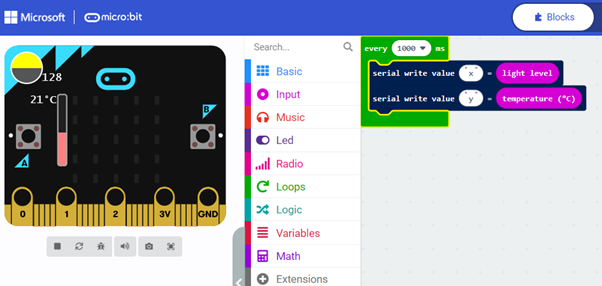
\includegraphics[width=10cm]{chapters/ChapterP2-datalog/figures/datalog1.png}
    \caption{Code for data logging}
    \label{fig:datalog1}
\end{figure}
 
\begin{figure}
    \centering
    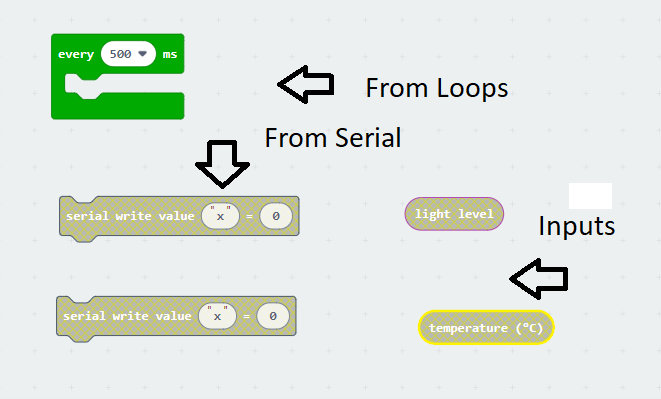
\includegraphics[width=10cm]{chapters/ChapterP2-datalog/figures/datalog2.png}
    \caption{Setting up step 1}
    \label{fig:datalogstep1}
\end{figure}


Figure 4.2 shows where various elements are in menu. To get the Serial ones you will need to open up the Advanced menu and then Serial menu options (see figure 4.3)
\begin{figure}
    \centering
    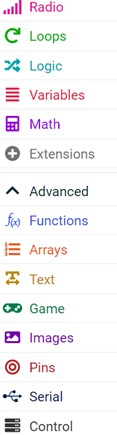
\includegraphics[width=10cm]{chapters/ChapterP2-datalog/figures/datalog3.png}
    \caption{Setting up step 2}
    \label{fig:datalogstep2}
\end{figure}
 
\begin{figure}
    \centering
    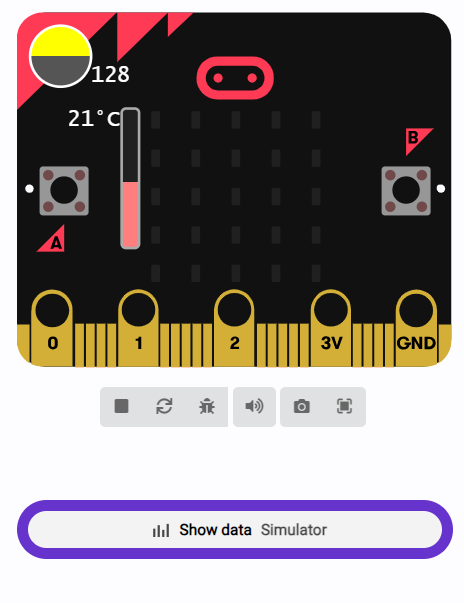
\includegraphics[width=10cm]{chapters/ChapterP2-datalog/figures/datalog4.png}
    \caption{Setting up step 3}
    \label{fig:datalogstep3}
\end{figure}

Once everything is set up under the similar microbit you will see another button “Show data Simulator” We can play with the microbit simulator toi simulate light and temperature levels; click on new data simulation button and graphs starts rolling across the screen – dag the temperature and light levels on the microbit simulator and you see the graphs change – it is logging the simulate data – it works!
Now for the fun bit.
Click on Download we need to pair the computer and microbit. Figures 4.5 to 4.8 show the steps.
 
\begin{figure}
    \centering
    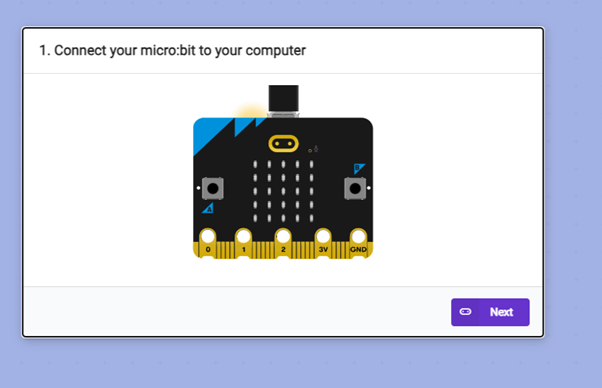
\includegraphics[width=10cm]{chapters/ChapterP2-datalog/figures/datalog5.png}
    \caption{Setting up step 4}
    \label{fig:datalogstep4}
\end{figure}
\begin{figure}
    \centering
    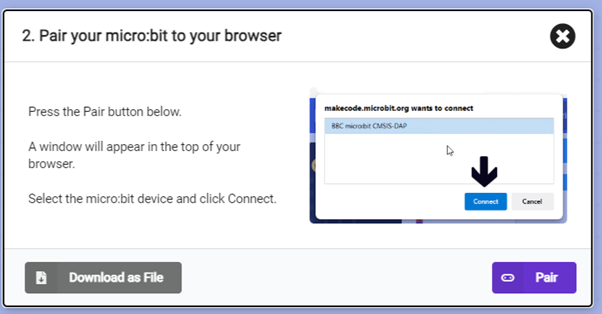
\includegraphics[width=10cm]{chapters/ChapterP2-datalog/figures/datalog6.png}
    \caption{Setting up step 5}
    \label{fig:datalogstep5}
\end{figure}

\begin{figure}
    \centering
    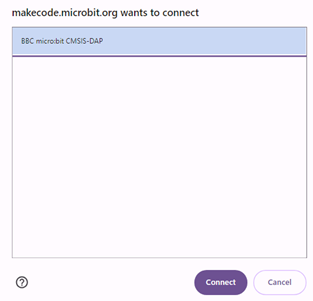
\includegraphics[width=10cm]{chapters/ChapterP2-datalog/figures/datalog7.png}
    \caption{Setting up step 6}
    \label{fig:datalogstep6}
\end{figure}
\begin{figure}
    \centering
    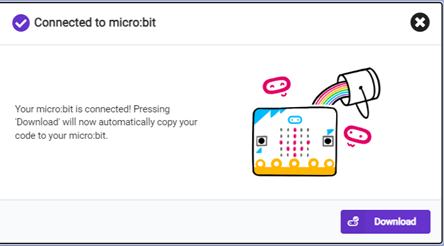
\includegraphics[width=10cm]{chapters/ChapterP2-datalog/figures/datalog8.png}
    \caption{Setting up step 7}
    \label{fig:datalogstep7}
\end{figure}

We can now take values from the real device. A new button should have appeared along with the “Show data Simulator” button; “Show data Device” Click on this button and instead os simulate data we get data from the  microbit (see figure 9)

 
\begin{figure}
    \centering
    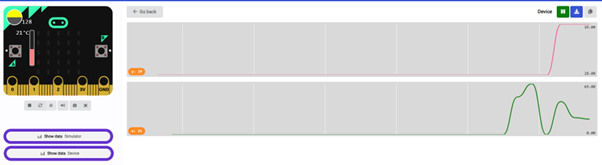
\includegraphics[width=10cm]{chapters/ChapterP2-datalog/figures/datalog9.png}
    \caption{Datalogging in action}
    \label{fig:datalogaction}
\end{figure}

So in figure 4.9 The top graph is light level the bottom is temperature taken from the room. Play with covering the sensor the LED grid and light levels change.

Collecting data is great, but we are taking it one step further logging the data over time To do this Click on the blue download button above the graphs to save the logged data as a CSV file. Once it is a CSV format it is yours to play with in other tools such as spreadsheets.


\subsection{Activity} 
-	how can this be more meaningful?
-	How do we do this with so a microbit can see data – some more remote monitoring (see \url{https://microbit.org/projects/make-it-code-it/makecode-wireless-data-logger/} )
-	How could you do this in Python

